When using machine learning models in real-world use cases, it is important to ensure those models are robust. If this is not the case they can be unreliable, wrong, or in the worst case attacked by adversaries. Finding and understanding the weaknesses, therefore, is important. Furthermore, understanding the weaknesses can also help us in finding better architectures that are less susceptible to these kinds of attacks.

Adversarial samples for machine learning models can be generated using the Fast Gradient Sign Method (FSGM)\cite{goodfellow2015explaining}. Originally proposed for image classification, it finds a small noise field that can be added to the image to generate an adversarial image. This adversarial image is then often incorrectly labeled with high confidence. An example of FSGM can be seen in figure \ref{adv_gibbon}. These adversarial samples prove to be useful during training, as they can act as regularizers, and improve the robustness of the model. \citeauthor{https://doi.org/10.48550/arxiv.1611.01236} show that these adversarial samples are also transferable to different models, even if they are trained on other datasets or have different architectures. This might make it possible to generate adversarial samples once and add them to the dataset, to make the dataset itself more robust.

\begin{figure*}[h]
    \centering
    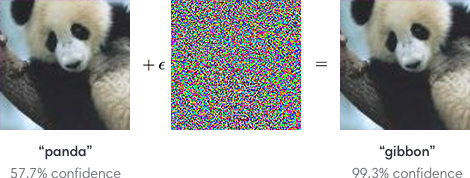
\includegraphics[width=0.9\textwidth]{figures/adversarial_img_1.png}
    \caption{Adversarial noise example from \protect\cite{goodfellow2015explaining}. Where $\epsilon=0.07$.}
    \label{adv_gibbon}
\end{figure*}

There has already been some research on adversarial examples targeted at image captioning \cite{https://doi.org/10.48550/arxiv.2107.03050,Hongge}. All of which attack the output of the model, often intendig to generate a specific output sentence. \citeauthor{Hongge} show that Show-and-Tell\footnote[1]{Show-and-Tell is the predecessor of S.A.T. without attention mechanism}\cite{showandtell} is susceptible to adversarial samples. The question then arises if the attention added in S.A.T. makes it harder to generate adversarial samples or if it opens up a new attack vector.

\subsection{Research Questions}
This research investigates the susceptibility of S.A.T. against adversarial samples that are visually close but generate completely different descriptions as output. A special focus is placed on what the attention in S.A.T. does and if it is an attack vector. When the attention is not focused on the important parts of the image for generating the caption, the model is blind to those parts therefore not being able to describe those parts. It is therefore interesting to investigate if the attention can be used against S.A.T.
Concretely this paper will try to answer the following questions:
\begin{itemize}
    \item Is S.A.T. susceptible to adversarial attacks using the Fast Gradient Sign Method?
    \item Can the attention of S.A.T. be abused by adversarial samples?
\end{itemize}
